\PassOptionsToPackage{colorlinks, unicode, linkcolor=tugreen}{hyperref}
\documentclass[compress, 9pt, aspectratio=1610, professionalfonts]{beamer}

\usepackage{fontspec}
\usepackage{polyglossia}
\setmainlanguage{english}

\usepackage{microtype}

\usepackage{mathtools}
\usepackage[
  math-style=ISO,
  bold-style=ISO,
  nabla=upright,
  partial=upright,
]{unicode-math}
\setmathfont{Tex Gyre Pagella Math}[Scale=MatchLowercase]

\usepackage{csquotes}
\usepackage[
  locale=UK,
  load-configurations=astronomy,
  per-mode=symbol-or-fraction,
]{siunitx}
\DeclareSIUnit{\year}{a}
\AtBeginDocument{%
  \sisetup{%
    math-rm=\mathrm,
  }
}

\usepackage{graphicx}
\usepackage{xcolor}
\colorlet{darkred}{red!80!black}

\usepackage{tikz}
\usetikzlibrary{positioning}
\usetikzlibrary{calc}
\usetikzlibrary{arrows}
\usetikzlibrary{arrows.meta}
\usepackage{pgfplots}

\usepackage[backend=biber, style=verbose]{biblatex}
\addbibresource{references.bib}
\usepackage{hyperref}

\usetheme{tudo}

\newcommand\fullscreenimage[2][]{{%
  \begin{frame}[plain]
    \begin{tikzpicture}[remember picture, overlay, shift=(current page.south west)]
      \fill[black] (0, 0) rectangle (\paperwidth, \paperheight);
      \node[anchor=center] at (current page.center) {%
        \includegraphics[
          width=\paperwidth,
          height=\paperheight,
          keepaspectratio,
        ]{#2}%
      };%
      \node[anchor=south east] at (current page.south east) {#1};%
    \end{tikzpicture}
  \end{frame}%
}}


\tikzset{%
  invisible/.style={opacity=0,text opacity=0},
  visible on/.style={alt={#1{}{invisible}}},
  alt/.code args={<#1>#2#3}{%
    \alt<#1>{\pgfkeysalso{#2}}{\pgfkeysalso{#3}} % \pgfkeysalso doesn't change the path
  },
}

\newcommand\freepicture[3]{%
  \begin{tikzpicture}[remember picture, overlay, shift=(current page.south west)]
    \node[anchor=center] at (#1\paperwidth, #2\paperheight) {#3};
  \end{tikzpicture}%
}

\newcommand\Photon{\ensuremath{\symup{γ}}}
\newcommand\Proton{\ensuremath{\symup{p}}}
\newcommand\Muon{\ensuremath{\symup{μ}}}


\author[M.\ Nöthe]{\textit{Maximilian Nöthe}, Kai Brügge for the FACT-Collaboration}
\date[20.2.2018]{HAP Workshop – Big Data Science in Astroparticle Research – 2018}
\title{FACT Open Data}
\titlegraphic{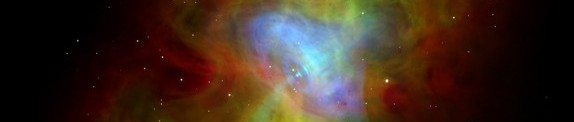
\includegraphics[width=\linewidth]{images/crab_title.jpg}}

\institute[%
  {
\includegraphics[height=\headerheight]{logos/fact.pdf}}%
  \hspace{1em}%
  {
\includegraphics[height=\headerheight]{logos/sfb876.pdf}}%
  \hspace{1em}%
  {
\includegraphics[height=\headerheight]{logos/e5logo.pdf}}%
]{
  {\includegraphics[height=0.75cm]{tu.pdf}}%
  \hspace{1em}%
  {
\includegraphics[height=0.75cm]{logos/ethz.pdf}}%
  \hspace{1em}%
  {
\includegraphics[height=0.75cm]{logos/isdc.pdf}}%
  \hspace{1em}%
  {
\includegraphics[height=0.75cm]{logos/uniwue.pdf}}%
}

\begin{document}
\begin{frame}
  \maketitle
\end{frame}

\begin{frame}{Overview}
  \begin{columns}[c, onlytextwidth]
    \begin{column}{0.66\textwidth}
      \linespread{1.5}
      \tableofcontents[hideallsubsections]
    \end{column}
    \hfill
    \begin{column}{0.33\textwidth}
      \raggedleft
      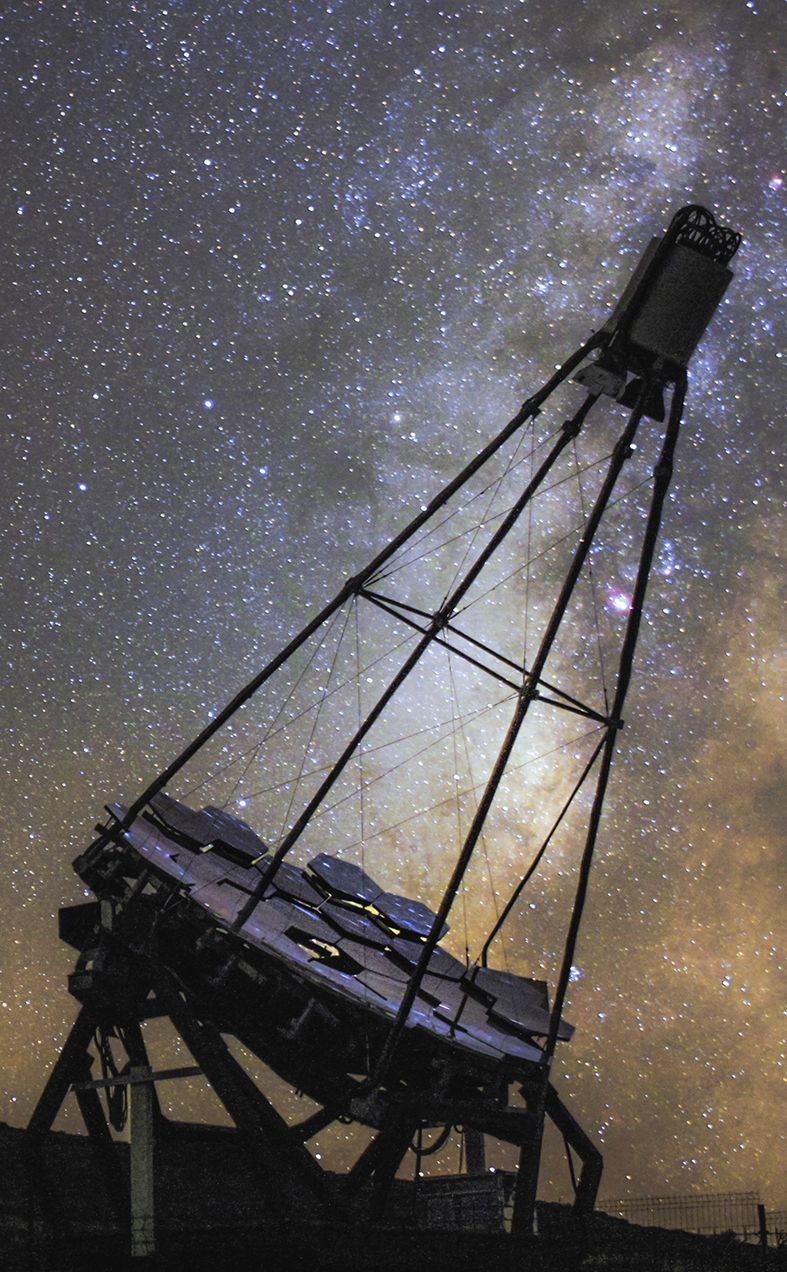
\includegraphics[height=0.85\textheight]{fact_claro_crop.jpg}\\
      {\tiny[Miguel Claro]}
    \end{column}
  \end{columns}
\end{frame}

\section{Introduction}
\begin{frame}
  \begin{center}
    \begin{tikzpicture}
      \large
\coordinate (mirror) at (4.1, 3.95);
\coordinate (cameracenter) at (8.4, 4.6);

\node[anchor=south west,inner sep=0] (background) at (0, 0) {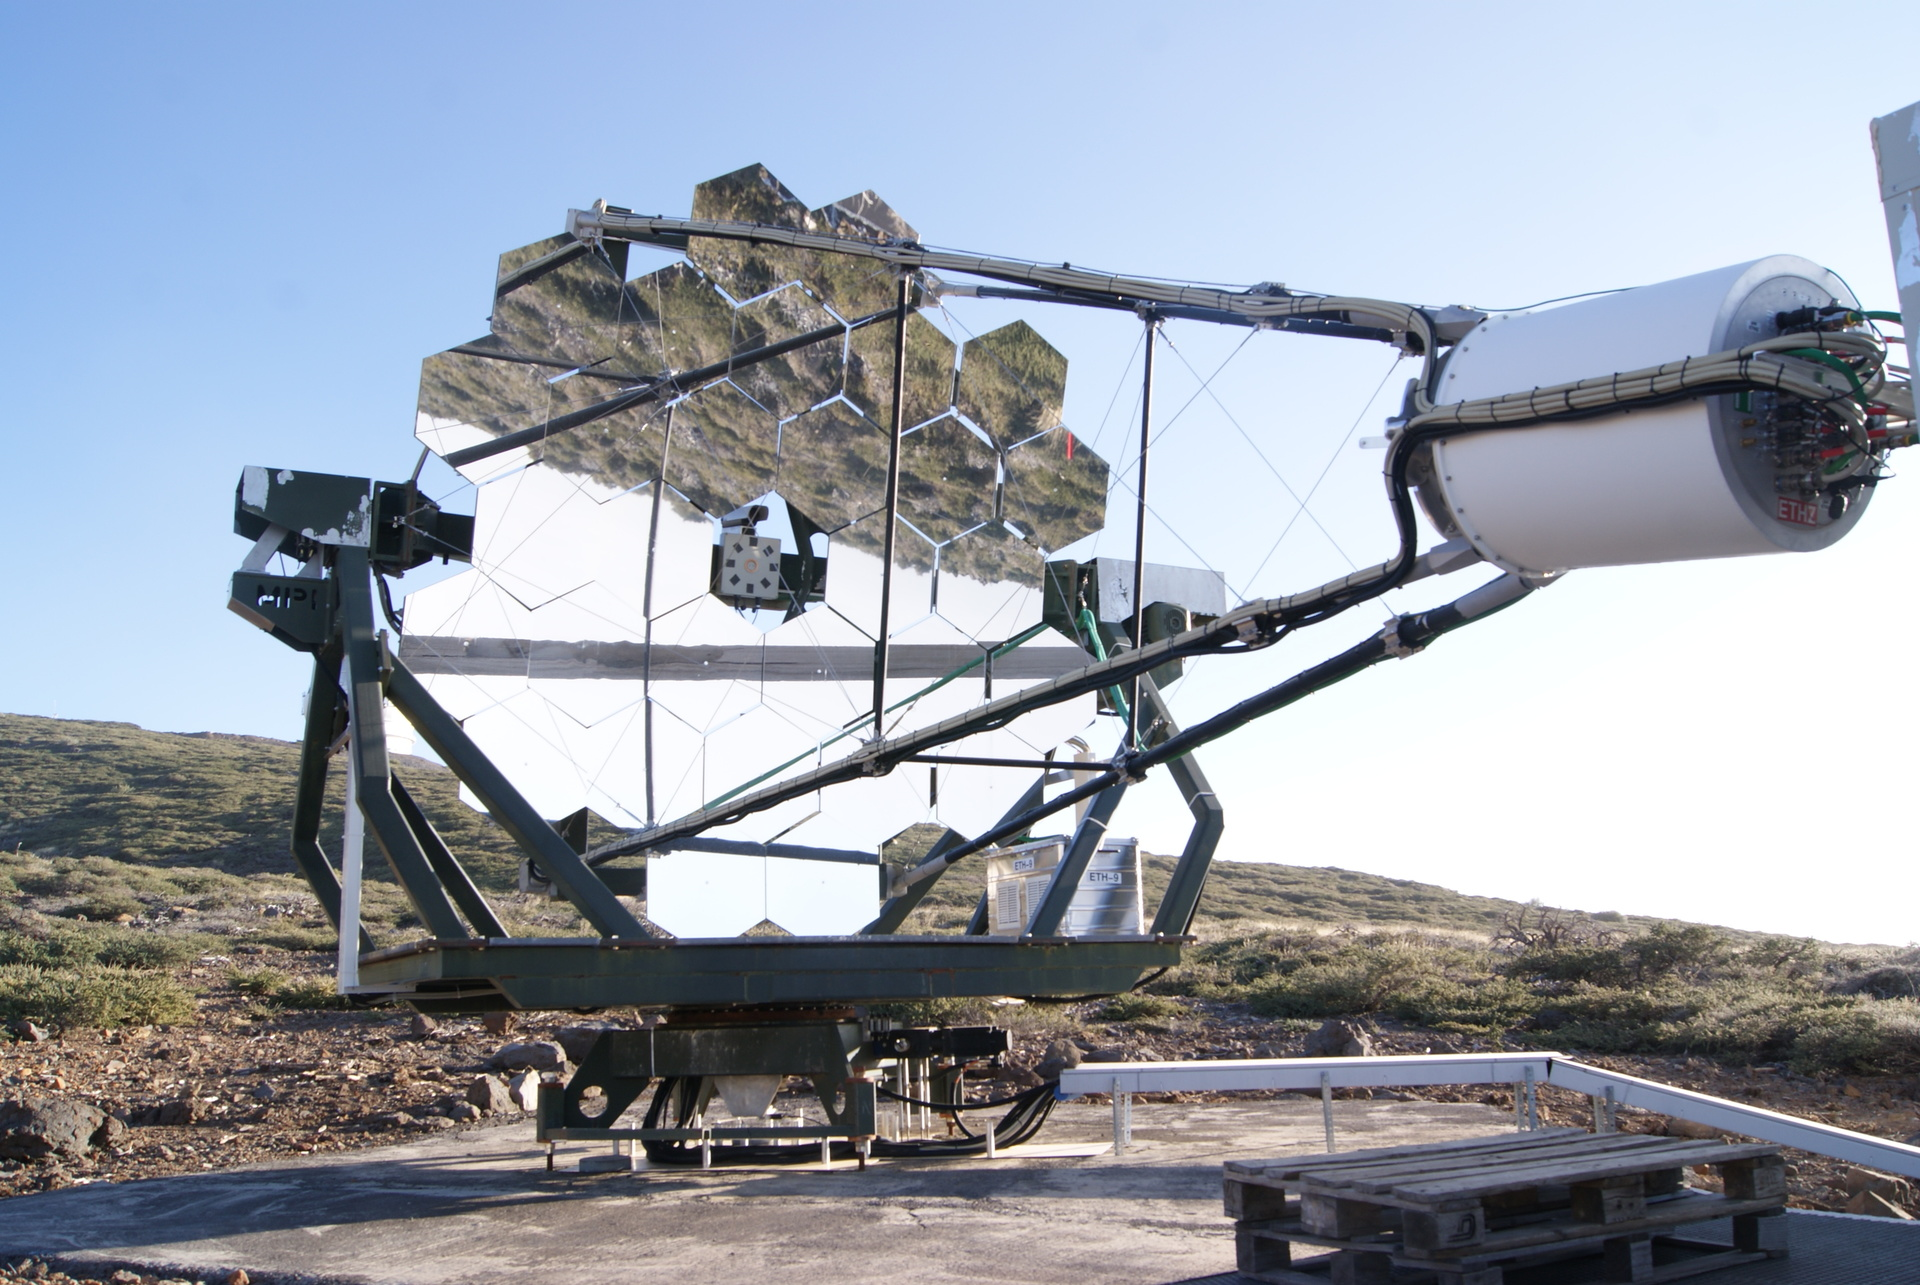
\includegraphics[height=0.92\textheight]{images/fact.jpg}};


\node[anchor=south west,inner sep=0] (camera) at (7, 0.5) {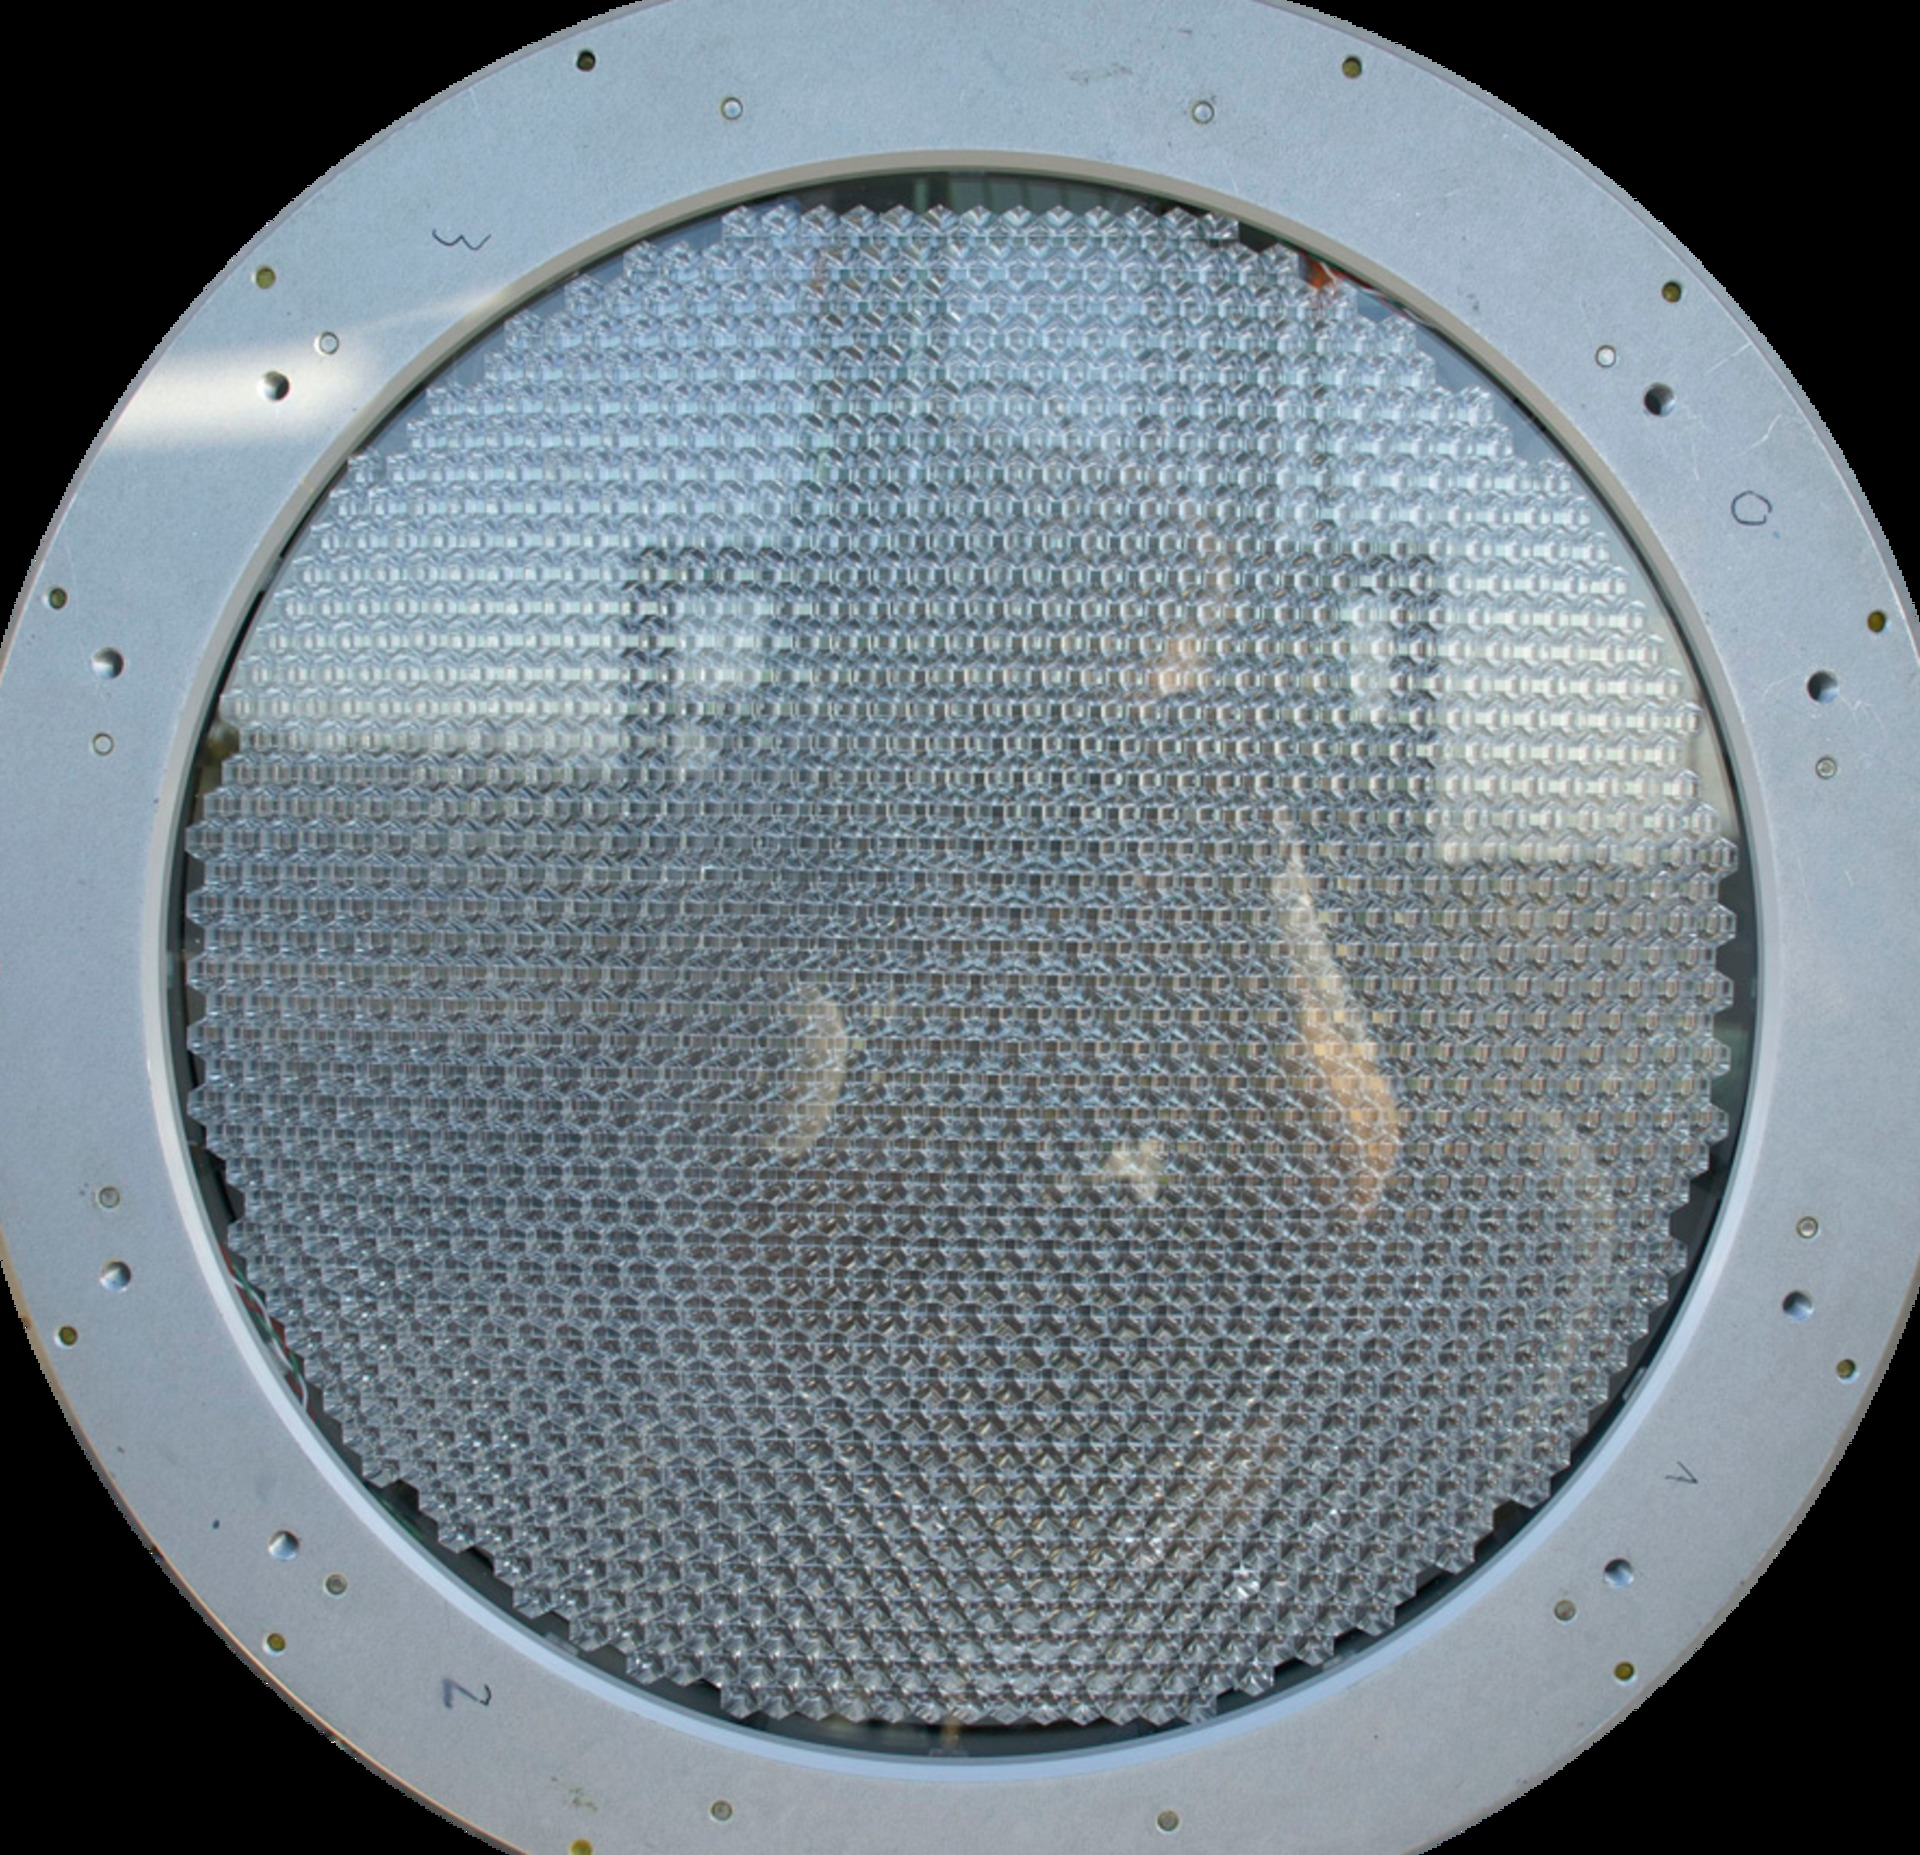
\includegraphics[width=0.2\textwidth]{images/camera.jpg}};



\draw[very thick,tugreen] (mirror) circle (2.05);
%\draw[thick,tugreen] (4,3.75) circle (0.05);
\draw[very thick,tugreen, rotate around={45:(mirror)}] ($(mirror)-(2.05,0)$) --
  ($(mirror)+(2.05,0)$)
  node[midway, above, black, fill=white, fill opacity=0.7, text opacity=1, rotate=45, rounded corners,]{$\diameter = \SI{3.8}{\meter}$};



\draw[very thick,tugreen] (cameracenter) ellipse (0.58 and 0.73);
%\draw[thick,tugreen] (7.9,4.4) circle (0.05);
\draw[very thick,tugreen] ($(cameracenter)-(0.58,0)$) to ($(camera.west)-(0.005*\textwidth,0)$);
\draw[very thick,tugreen] ($(cameracenter)+(0.58,0)$) to ($(camera.east)+(0.005*\textwidth,0)$);
\draw[very thick,tugreen] (camera.center) circle (0.105\textwidth);

\node[black,anchor=south west, fill=white, rounded corners] at (0.6,0.15) {\textbf{Roque des los Muchachos, La Palma}};


\node[black,anchor=center,text centered, fill=white, fill opacity=0.7, text opacity=1, rounded corners] at (camera.center) {\textbf{1440 Pixel}};
\node[black,anchor=east,text centered] at (9.9,6.4) {\textbf{1 Pixel = 1 SiPM = 3600 G-APDs}};

    \end{tikzpicture}
  \end{center}
\end{frame}

\section{Dataset Overview}
\begin{frame}[c]{The Dataset}
  \begin{columns}[onlytextwidth]
    \begin{column}{0.55\textwidth}      
      \begin{itemize}
        \item Crab Observations from November 2013
        \item Point-source gamma-ray simulations
        \item Diffuse gamma-ray simulations
        \item Diffuse proton simulations
        \item Available in different formats and multiple analysis stages
      \end{itemize}
    \end{column}
    \hfill
    \begin{column}{0.4\textwidth}      
      \hfill
      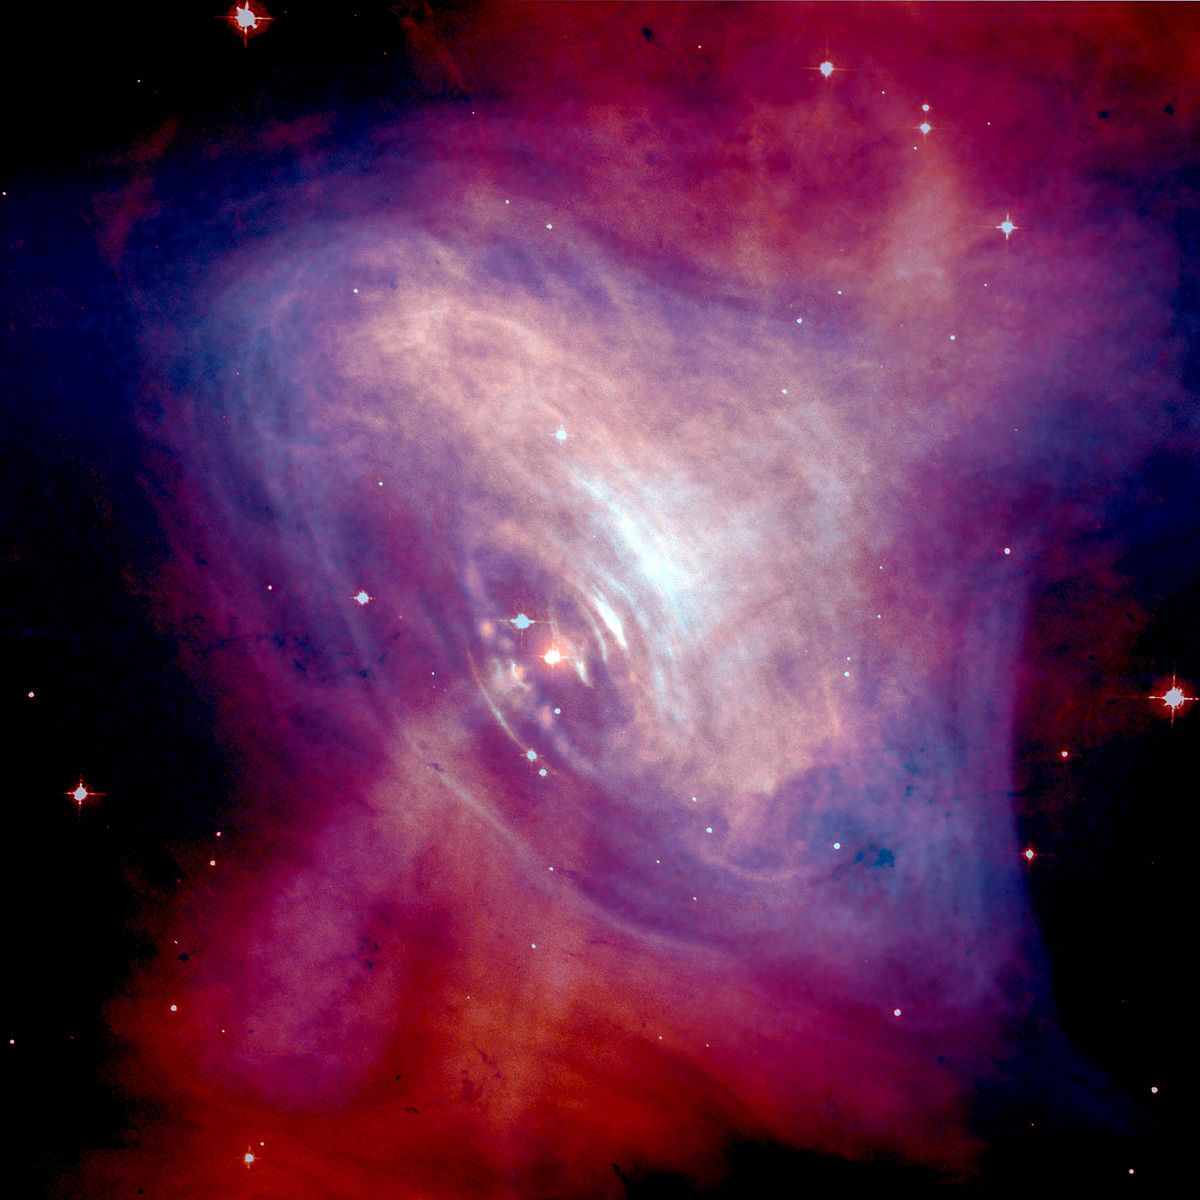
\includegraphics[width=0.75\textheight]{images/crab_chandra.jpg}
    \end{column}
  \end{columns}
  \vspace{0.5cm}
  \begin{center}
    \LARGE\url{https://fact-project.org/data}
  \end{center}
\end{frame}

\begin{frame}[c]{Observations}
  \begin{columns}[onlytextwidth]
    \begin{column}{0.475\textwidth}      
      \begin{itemize}
        \item \num{17.7} hours of Crab Nebula observations
        \item Good environmental conditions
        \item Zenith distance between \ang{6} and \ang{30}
      \end{itemize}
      \vspace{0.25cm}
      \begin{center}
        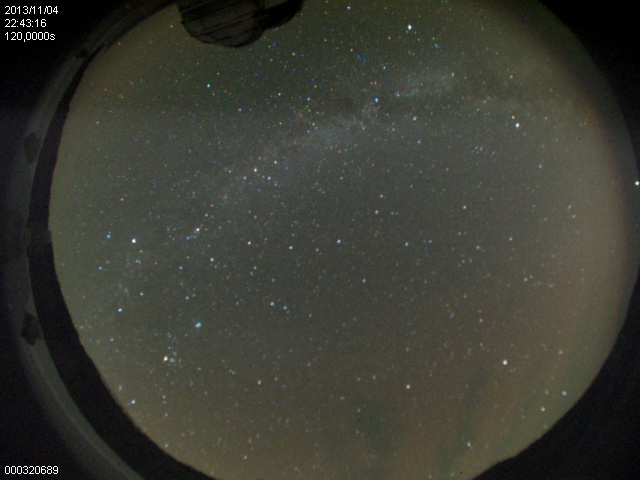
\includegraphics[width=0.75\linewidth]{images/gtc.jpg}
      \end{center}
    \end{column}
    \hfill
    \begin{column}{0.475\textwidth}      
      \includegraphics{build/plots/zenith.pdf}
    \end{column}
  \end{columns}
  
\end{frame}

\begin{frame}[t]{Simulations}
  \begin{itemize}
    \item CORSIKA for air shower simulations
    \item CERES for FACT detector response simulations
  \end{itemize}

  \vspace{1cm}

  \begin{columns}[onlytextwidth]
    \begin{column}{0.475\textwidth}
      \textcolor{tugreen}{\Large Gammas}
      \begin{description}[Triggered Events]
        \item[Energy Range] \SI{200}{\GeV} – \SI{50}{\TeV}
        \item[Spectral Slope] \num{-2.7}
        \item[Max. Impact] \SI{270}{\meter}
        \item[Zenith Distance] \ang{0} – \ang{30}
        \item[CORSIKA Events] \num{12000000}
        \item[Triggered Events] \num{1914812}
      \end{description}
    \end{column}
    \hfill
    \begin{column}{0.475\textwidth}
      \textcolor{tugreen}{\Large Protons}
      \begin{description}[Triggered Events]
        \item[Energy Range] \SI{100}{\GeV} – \SI{200}{\TeV}
        \item[Spectral Slope] \num{-2.7}
        \item[Max. Impact] \SI{400}{\meter}
        \item[Zenith Distance] \ang{0} – \ang{30}
        \item[CORSIKA Events] \num{780046520}
        \item[Triggered Events] \num{509652}
      \end{description}
    \end{column}
  \end{columns}
\end{frame}

\begin{frame}[t]{A FACT Analysis}
  \begin{columns}[onlytextwidth]
    \begin{column}{0.475\textwidth}
      Classical IACT Analysis Chain
      \begin{enumerate}
        \item Raw Data Calibration
        \item Removal of electronic artifacts
        \item Extraction of number of photons and mean arrival times for each pixel
        \item Image parameterization
        \item Reconstruction of particle properties
          \begin{itemize}
            \item Energy
            \item Origin
            \item Particle type (\Photon, \Proton, \Muon)
          \end{itemize}
      \end{enumerate}
    \end{column}
    \hfill
    \begin{column}{0.475\textwidth}%
      \only<1>{\includegraphics{build/plots/drs_calib.pdf}}%
      \only<2>{\includegraphics{build/plots/spikes.pdf}}%
      \only<3>{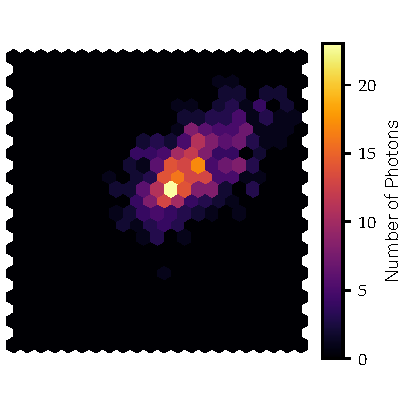
\includegraphics{images/hillas_1.pdf}}%
      \only<4>{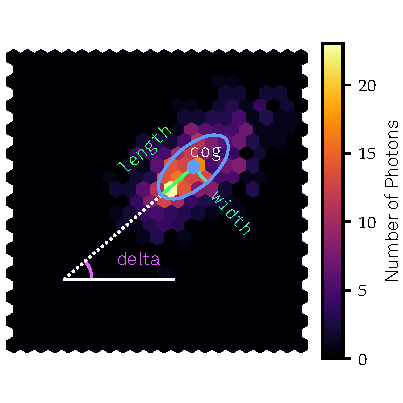
\includegraphics{images/hillas_2.pdf}}%
    \end{column}%
  \end{columns}
\end{frame}

\section{Data Formats}
\begin{frame}[t]{Raw Data}
  \begin{itemize}
    \item FACT observations are stored in custom compressed FITS Files called \texttt{zfits}\\
    \item Readers are available for
      \begin{description}
        \item[Python] \url{https://github.com/fact-project/zfits} 
        \item[Java] \url{https://github.com/fact-project/fact-tools} 
        \item[C++ (ROOT)] \url{https://trac.fact-project.org/browser/trunk/Mars} 
      \end{description}
    \item FACT-Tools can be easily used to convert \texttt{zfits} to standard FITS
    \item Simulations are stored in standard, gzipped FITS Files
    \item Raw Data consists of a single array of length $1440 \times 300$ ($N_\text{Pixels} \times N_\text{Slices}$)

      \vspace{0.2cm}
      \begin{center}
        \begin{tikzpicture}
          \foreach \i in {0,...,2} {
            \node[anchor=west, minimum width=0.5cm, minimum height=0.5cm, fill=blue!20, draw=black] at (\i * 0.5cm, 0) {\tiny \i};
          }
          \node[anchor=west, minimum width=0.5cm, minimum height=0.5cm] at (1.5cm, 0) {$\cdots$};
          \foreach \j in {298,299} {
            \node[anchor=west, minimum width=0.5cm, minimum height=0.5cm, fill=blue!20, draw=black] at (\j * 0.5cm - 147cm, 0) {\tiny \j};
          }
          \foreach \i in {0,...,2} {
            \node[anchor=west, minimum width=0.5cm, minimum height=0.5cm, fill=green!20, draw=black] at (\i * 0.5cm + 3cm, 0) {\tiny \i};
          }
          \node[anchor=west, minimum width=0.5cm, minimum height=0.5cm] at (4.5cm, 0) {$\cdots$};
          \foreach \j in {298,299} {
            \node[anchor=west, minimum width=0.5cm, minimum height=0.5cm, fill=green!20, draw=black] at (\j * 0.5cm - 144cm, 0) {\tiny \j};
          }
          \node[anchor=west, minimum width=0.5cm, minimum height=0.5cm] at (6cm, 0) {$\cdots$};
          \node at (1.5cm, -0.5cm) {Pixel 0};
          \node at (4.5cm, -0.5cm) {Pixel 1};
        \end{tikzpicture}
      \end{center}

      \vspace{0.2cm}
      \begin{center}
        \LARGE 0.9\,TB observations, 1.1\,TB simulations
      \end{center}
  \end{itemize}
    
  \begin{center}
    \small See: \cite{zfits}
  \end{center}
\end{frame}

\begin{frame}[c]{Photon Stream}
  \begin{columns}[onlytextwidth]
    \begin{column}{0.475\textwidth}
      \begin{itemize}
        \item The FACT Camera has single photon resolution
        \item Each photon produces a known pulse shape 
        \item Multiple photons just superimpose
        \item[→] Reconstruct the arrival time of each individual photon by subtracting pulses until a flat line is reached
        \item \emph{Much} smaller file size compared to raw data
        \item All FACT Data $\approx{}$ 8\,TB
      \end{itemize}
      \begin{center}
        \small See: \cite{photonstream}
      \end{center}
    \end{column}
    \begin{column}{0.475\textwidth}
      \includegraphics{build/plots/phs.pdf}
    \end{column}
  \end{columns}
\end{frame}

\section{FACT-Tools Standard Analysis}
\begin{frame}[t]{FACT-Tools}
  \begin{itemize}
    \item Extension of the \texttt{streams}-Framework to analyze FACT data
    \item Developed at TU Dortmund and ETHZ
    \item Also performs photonstream extraction
  \end{itemize}

  \vspace{0.25cm}
  \begin{center}
    \Large\url{https://github.com/fact-project/fact-tools}
  \end{center}

  \vspace{0.25cm}
  \begin{center}
    \begin{tikzpicture}[scale=1, transform shape]
      \tikzstyle{box}=[draw=black!50,rectangle, minimum height=1.75cm, minimum width=2cm, text width=2cm, text centered]

\begin{scope}[shift={(0.5,0.25)}]
\draw (0.3,-0.35) -- (0.0,-1);
\draw (0.5,-0.35) -- (0.8,-1);

\begin{scope}[rotate=-20]
\draw (0.15,-0.1) -- (0.4,0.55);
\draw (0.85,-0.1) -- (0.6,0.55);

\node (CAM) at (0.5,0.6) {};

\draw[fill=black!10] (0.4,0.45) -- (0.6,0.45) -- (0.6,0.7) -- (0.4,0.7) -- (0.4,0.45);

\fill[fill=black!10] (0,0) to[out=300,in=240] (1,0) -- (0,0);
\draw (0,0) to[out=300,in=240] (1,0) -- (0,0);

\end{scope}
\end{scope}

\begin{scope}[shift={(1.85,-0.2)}]
\draw[draw=tugreen,fill=tugreen!50] (0.2,0) -- (0.5,0) -- (0.5,-0.1) -- (0.75,0.15) -- (0.5,0.4) -- (0.5,0.3) -- (0.2,0.3) -- (0.2,0);
\end{scope}

\begin{scope}[shift={(5.05,-0.2)}]
\draw[draw=tugreen,fill=tugreen!50] (0.2,0) -- (0.5,0) -- (0.5,-0.1) -- (0.75,0.15) -- (0.5,0.4) -- (0.5,0.3) -- (0.2,0.3) -- (0.2,0);
\end{scope}

\begin{scope}[shift={(8.05,-0.2)}]
\draw[draw=tugreen,fill=tugreen!50] (0.2,0) -- (0.5,0) -- (0.5,-0.1) -- (0.75,0.15) -- (0.5,0.4) -- (0.5,0.3) -- (0.2,0.3) -- (0.2,0);
\end{scope}

\begin{scope}[shift={(11.05,-0.2)}]
\draw[draw=tugreen,fill=tugreen!50] (0.2,0) -- (0.5,0) -- (0.5,-0.1) -- (0.75,0.15) -- (0.5,0.4) -- (0.5,0.3) -- (0.2,0.3) -- (0.2,0);
\end{scope}
%
%\begin{scope}[shift={(14.05,-0.2)}]
%\draw[draw=tugreen,fill=tugreen!50] (0.2,0) -- (0.5,0) -- (0.5,-0.1) -- (0.75,0.15) -- (0.5,0.4) -- (0.5,0.3) -- (0.2,0.3) -- (0.2,0);
%\end{scope}

% \begin{scope}[shift={(17.05,-0.2)}]
% \draw[draw=tugreen,fill=tugreen!50] (0.2,0) -- (0.5,0) -- (0.5,-0.1) -- (0.75,0.15) -- (0.5,0.4) -- (0.5,0.3) -- (0.2,0.3) -- (0.2,0);
% \end{scope}


\node[box] (CAL) at (4,0) {\textsf{Calibration}};
\node[box] (EXT) at (7,0) {\textsf{Signal extraction}};
\node[box] (CLEAN) at (10,0) {\textsf{Image cleaning}};
\node[box] (PAR) at (13,0) {\textsf{Parameterization}};
%\node[box] (SEP) at (16,0) {\small \textsf{Gamma-Proton classification}};
% \node[box] (EST) at (19,0) {\textsf{Flux Estimation}};


% \draw[thick,black!60,<->] (FEAT.north) + (0.1,0) -- +(0.1, 0.25) -- +(3, 0.25) -- (SEP.north);
% \draw[thick,black!60,<->] (FEAT.south) -- +(0,-0.25) -- +(6,-0.25) -- (SPEC.south);
%
% \draw[thick,black!60,<->] (CAL.north) -- +(0, 0.25) -- +(2.8,0.25) -- +(2.8,0);
% \draw[thick,black!60,<->] (CAL.south) -- +(0,-0.25) -- +(-3.1,-0.25) -- +(-3.1,0);

    \end{tikzpicture}
  \end{center}
\end{frame}

\begin{frame}[c, fragile]{Higher-Level Analysis}
  \begin{itemize}
    \item We use the Scientific Python Stack
    \item \texttt{scikit-learn} models for particle classification, energy estimation and reconstruction of origin
  \end{itemize}

  \vspace{0.25cm}
  
  Example analysis on the open data sample:

  \begin{verbatim}
  $ git clone https://github.com/fact-project/open_crab_sample_analysis
  $ pip install -r requirements.txt
  $ make
  \end{verbatim}

  This will download the data, train models, apply them and produce a $θ²$ plot for the source detection.

\end{frame}

\begin{frame}[t]{Result}
  \begin{center}
    \includegraphics{build/plots/theta2.pdf}
  \end{center}
\end{frame}

\section{Outlook \& Conclusion}

\begin{frame}[t]{Deep Learning}
  \begin{columns}[onlytextwidth]
    \begin{column}{0.55\textwidth}
      \begin{itemize}
        \item Ongoing efforts to try deep learning on this dataset
        \item Using photonstream representation
        \item Reducing the hexgrid and time domain to square images
      \end{itemize}

      See: \url{https://github.com/mackaiver/cnn_cherenkov}
    \end{column}
    \begin{column}{0.4\textwidth}
      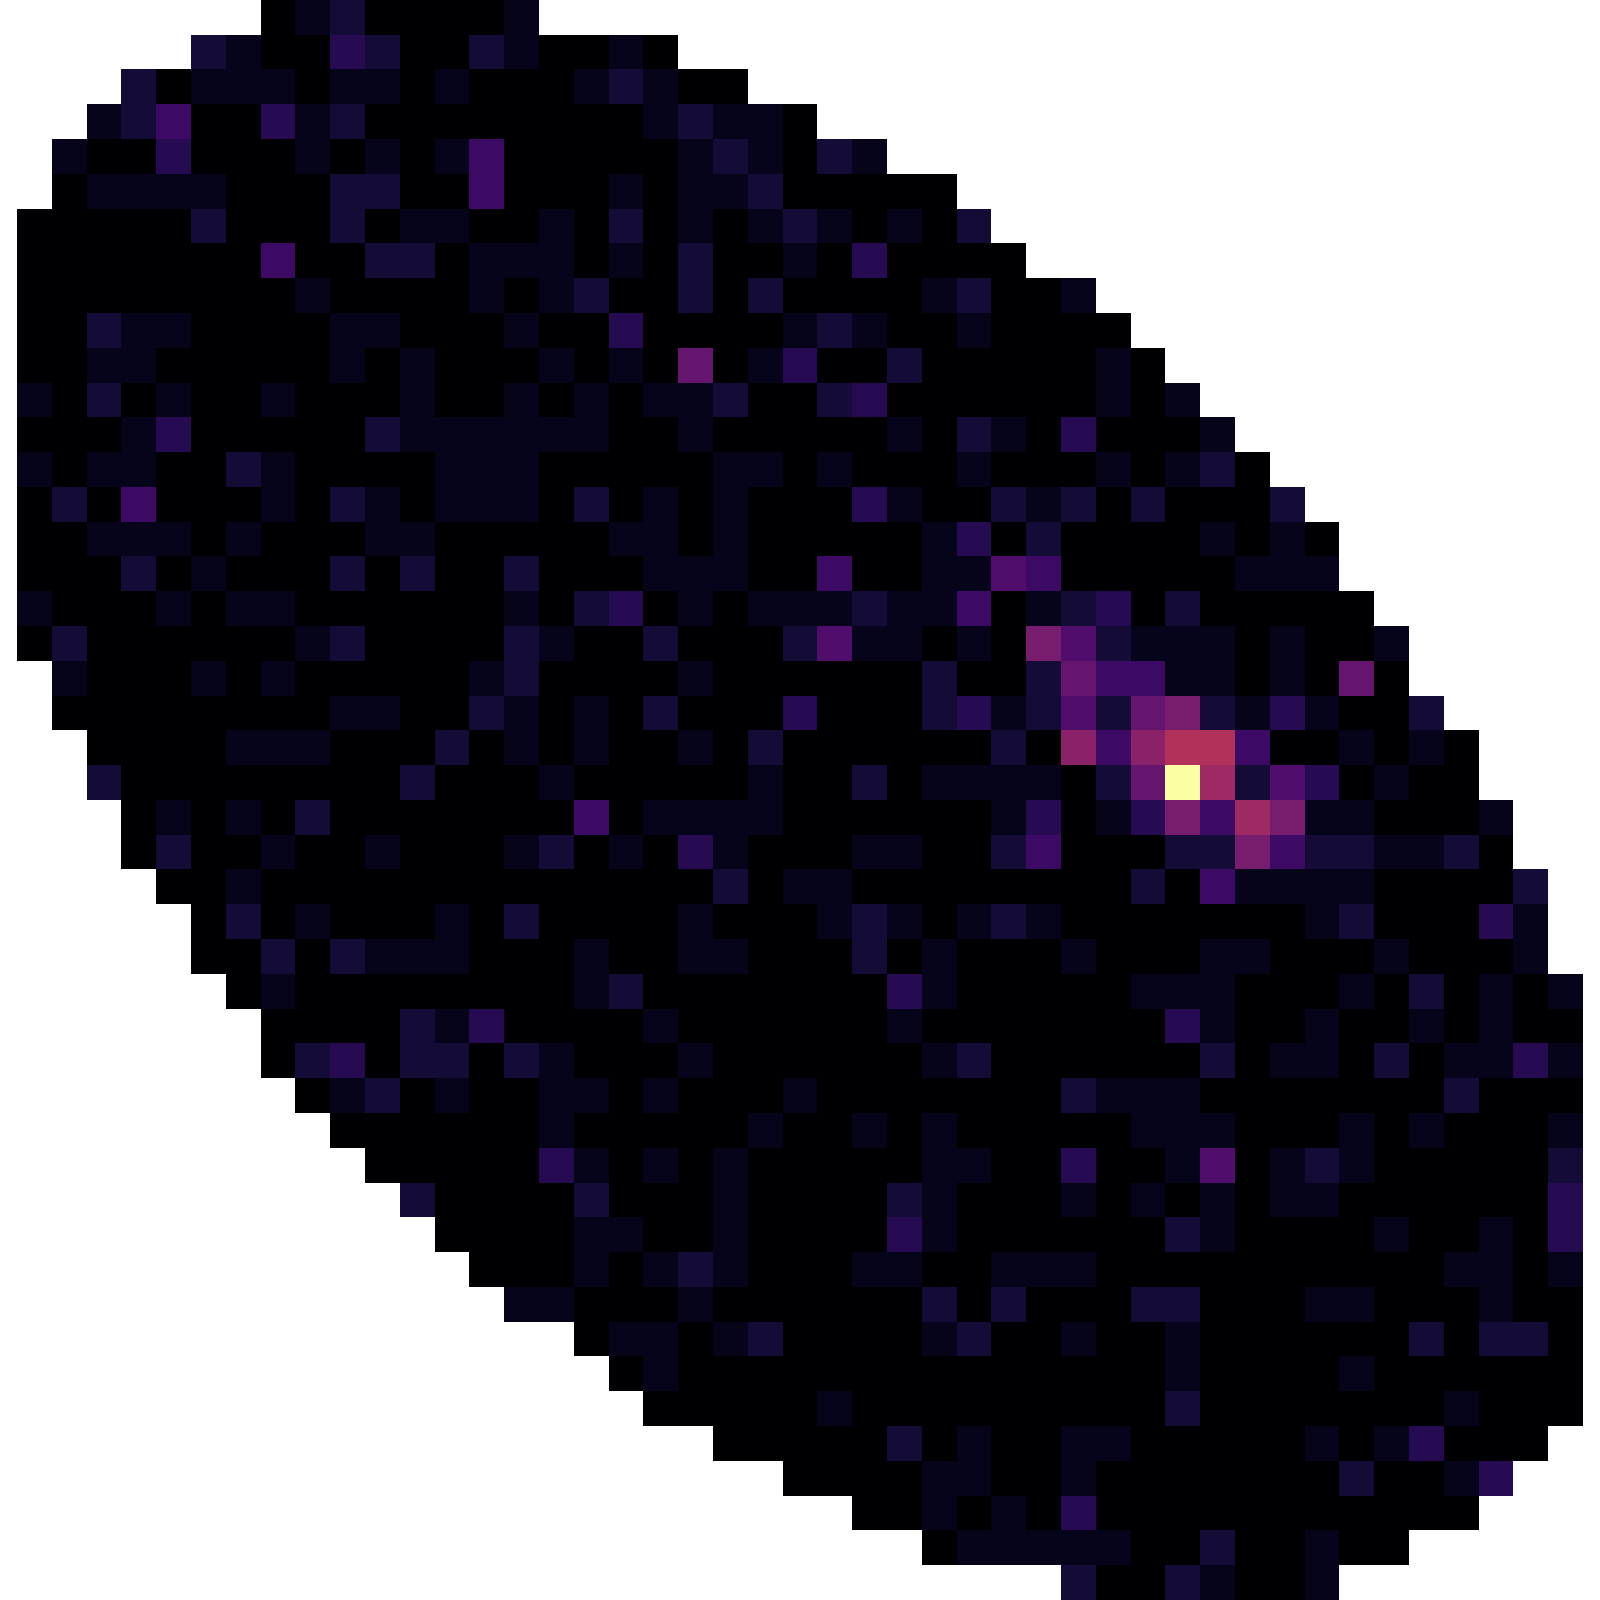
\includegraphics[width=\textwidth]{images/shower_skewed.png}
    \end{column}
  \end{columns}
\end{frame}

\begin{frame}[c]{Conclusions}
  \begin{itemize}
    \item From the start, FACT made results of he Quick Look Analysis publicly available \url{https://fact-project.org/monitoring}
    \item In November, FACT released a dataset of Crab observations, from the raw data up.
    \item Accompanied by extensive simulations.
    \item FACT-Tools standard analysis has \SI{23.8}{σ} on this dataset
    \item Use it for education and outreach!
    \item Many possibilities including Deep Learning, Spectrum Estimation, etc.
    \item We are planning on releasing more data in the future.
  \end{itemize}
\end{frame}

\end{document}
